\documentclass{standalone}
\usepackage{pgfplots}
\pgfplotsset{compat=1.18}
\usepgfplotslibrary{fillbetween}
\usetikzlibrary{patterns.meta}
\renewcommand{\familydefault}{\sfdefault}

\definecolor{myDarkGray}{gray}{0.3}  
\definecolor{myMidGray}{gray}{0.55}   
\definecolor{myLightGray}{gray}{0.75}  

\begin{document}
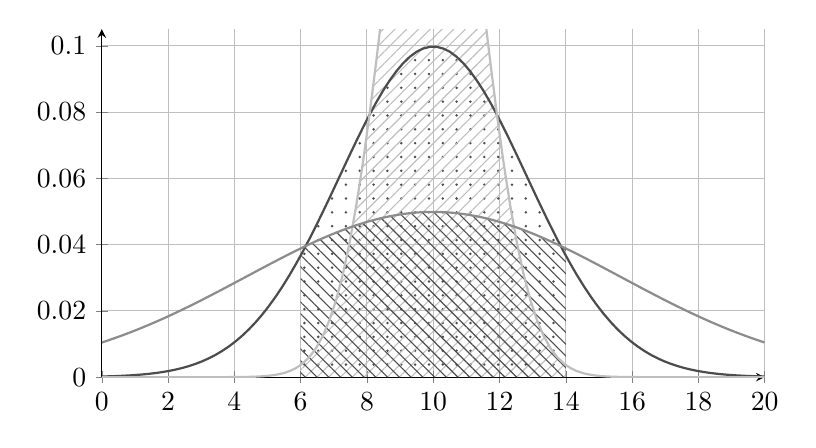
\begin{tikzpicture}
\begin{axis}[
    axis lines = left,
    grid=major,
    xlabel style={
        at={(ticklabel* cs:1)}, 
        anchor=north, 
        yshift=12pt},
    ylabel style={
        at={(ticklabel* cs:1)}, 
        anchor=north east,
        rotate=-90, 
        xshift=28pt,
        yshift=10pt},   
    scaled y ticks=false,
    y tick label style={
        /pgf/number format/fixed,
        /pgf/number format/precision=2,
    },
    xtick={0, 2, ..., 20},
     ymin=0, ymax=0.105,
    ytick={0,0.02,...,0.1},
    samples=100,
    domain=0:20,
    height=6cm,
    width=10cm,
    no markers,
    every axis plot/.append style={thick},
]
    %Kurven
    \addplot[name path=midcurve, myDarkGray] 
        {1/(4*sqrt(2*pi)) * exp(-((x-10)^2)/(16))};
    \addplot[name path=leftcurve, myLightGray] 
        {1/(2*sqrt(2*pi)) * exp(-((x-10)^2)/(4))};
    \addplot[name path=rightcurve, myMidGray] 
        {1/(8*sqrt(2*pi)) * exp(-((x-10)^2)/(64))};

    %unischtbare Linie auf der x-Achse
    \path[name path=axis] (6,0) -- (14,0);

    %Flächen
    \addplot[
        pattern color=myDarkGray,
        pattern={Dots[distance=5pt]}
    ] fill between [
        of=midcurve and axis,
        soft clip={domain=6:14}
    ];
    
    \addplot[
        pattern color=myLightGray,
        pattern={Lines[angle=45]}
    ] fill between [
        of=leftcurve and axis,
        soft clip={domain=6:14}
    ];

    \addplot[
        pattern color=myDarkGray,
        pattern={Lines[angle=135]}
    ] fill between [
        of=rightcurve and axis,
        soft clip={domain=6:14}
    ];







\end{axis}
\end{tikzpicture}
\end{document}
